\documentclass{article}
\usepackage{amsmath}
\usepackage{graphicx}
\usepackage{float}
\usepackage{hyperref}
\usepackage{fancyvrb}
\usepackage{matlab-prettifier}
\setlength{\parindent}{0pt}
\graphicspath{{../images/}}

\title{CS663: Digital Image Processing - Homework 2}
\author{Harsh $\vert$ Pranav $\vert$ Swayam} 
\date{September 6, 2024}

\begin{document}

\maketitle
\section{Homework 2 - Question 8}

\subsection*{(a)}

\begin{figure}[!htb]
    \centering
    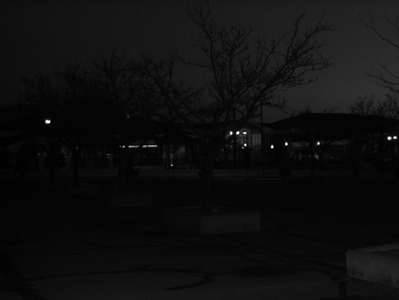
\includegraphics[width = 0.5\textwidth]{LC1.png}
    \caption{Original \texttt{LC1}}
\end{figure}

\begin{figure}[!htb]
    \centering
    \begin{minipage}[b]{0.45\textwidth}
        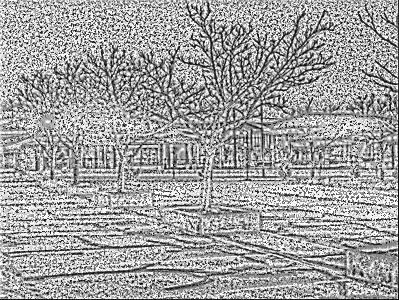
\includegraphics[width=\textwidth]{LC1_local_7.jpg}
        \caption{7x7 local histogram}
    \end{minipage}
    % \hfill
    \begin{minipage}[b]{0.45\textwidth}
        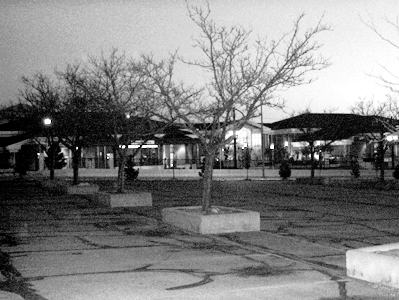
\includegraphics[width=\textwidth]{LC1_global.png}
        \caption{Global histogram}
    \end{minipage}
    % \hfill
\end{figure}

Here the 7X7 bin local histogram is not good, although on the pointed tree it gives more sharper edges of the branch of the tree in comparison to the global image.

\begin{figure}[!htb]
    \centering
    \begin{minipage}[b]{0.45\textwidth}
        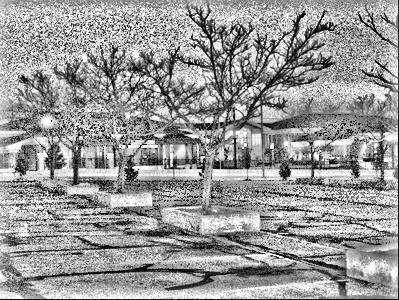
\includegraphics[width=\textwidth]{LC1_local_31.jpg}
        \caption{31x31 local histogram}
    \end{minipage}
    % \hfill
    \begin{minipage}[b]{0.45\textwidth}
        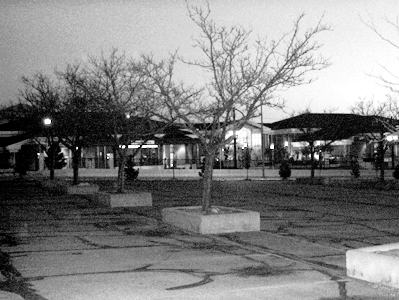
\includegraphics[width=\textwidth]{LC1_global.png}
        \caption{Global histogram}
    \end{minipage}
    % \hfill
\end{figure}

Here, the 31X31 bin local histogram image appears better than the 7X7, and the ground lines are more visible and are more darker/sharper than the ground which is missing in global.

\begin{figure}[!htb]
    \centering
    \begin{minipage}[b]{0.45\textwidth}
        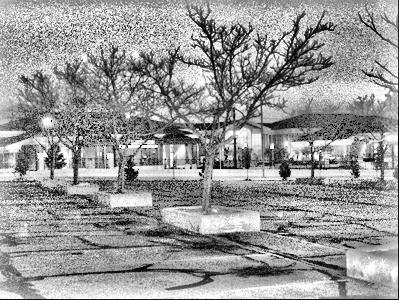
\includegraphics[width=\textwidth]{LC1_local_51.jpg}
        \caption{51x51 local histogram}
    \end{minipage}
    % \hfill
    \begin{minipage}[b]{0.45\textwidth}
        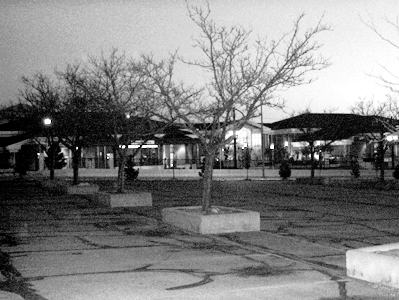
\includegraphics[width=\textwidth]{LC1_global.png}
        \caption{Global histogram}
    \end{minipage}
    % \hfill
\end{figure}

In the 51X51 bin local histogram, the window of house is clearly visible in contrast to the global histogram. And some specific regions got darker/sharper as compared to 31x31.

\begin{figure}[!htb]
    \centering
    \begin{minipage}[b]{0.45\textwidth}
        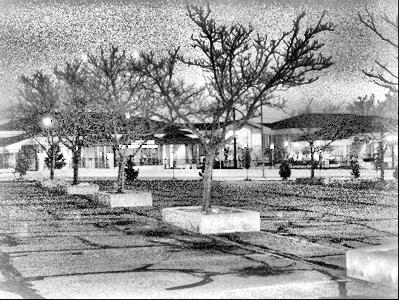
\includegraphics[width=\textwidth]{LC1_local_71.jpg}
        \caption{71x71 local histogram}
    \end{minipage}
    % \hfill
    \begin{minipage}[b]{0.45\textwidth}
        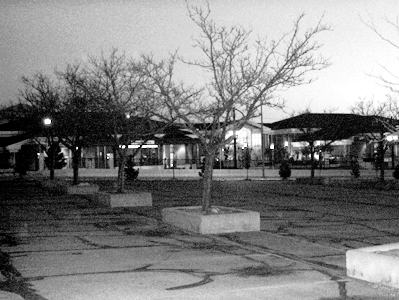
\includegraphics[width=\textwidth]{LC1_global.png}
        \caption{Global histogram}
    \end{minipage}
    % \hfill
\end{figure}

Now, the 71X71 bin gets better and has reached closer to the global histogram. The earlier sections that we defined above have become much more sharper and precise in the local histogram against the global counterpart.

% \newpage
\subsubsection*{(b)}

\begin{figure}[!htb]
    \centering
    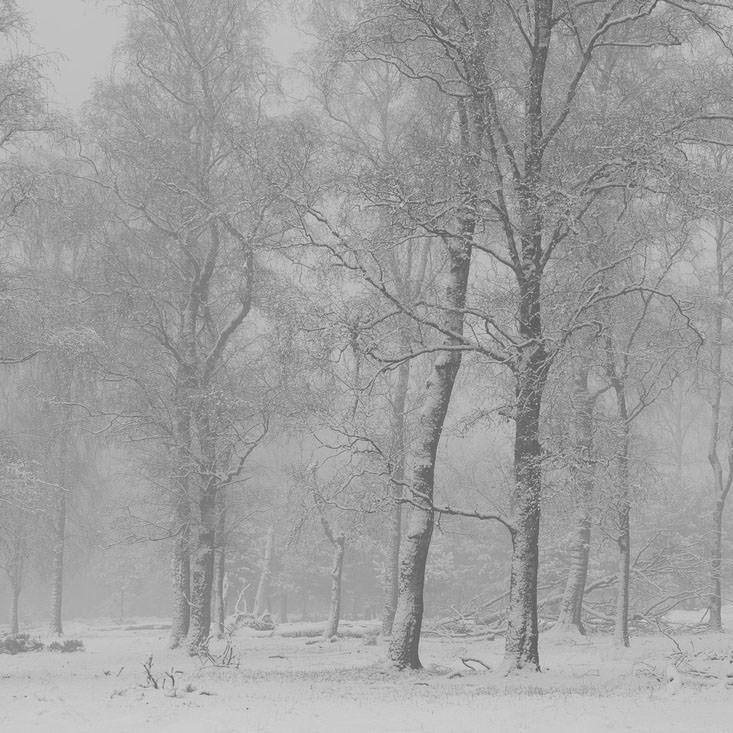
\includegraphics[width = 0.5\textwidth]{LC2.jpg}
    \caption{Original \texttt{LC2}}
\end{figure}

\begin{figure}[!htb]
    \centering
    \begin{minipage}[b]{0.45\textwidth}
        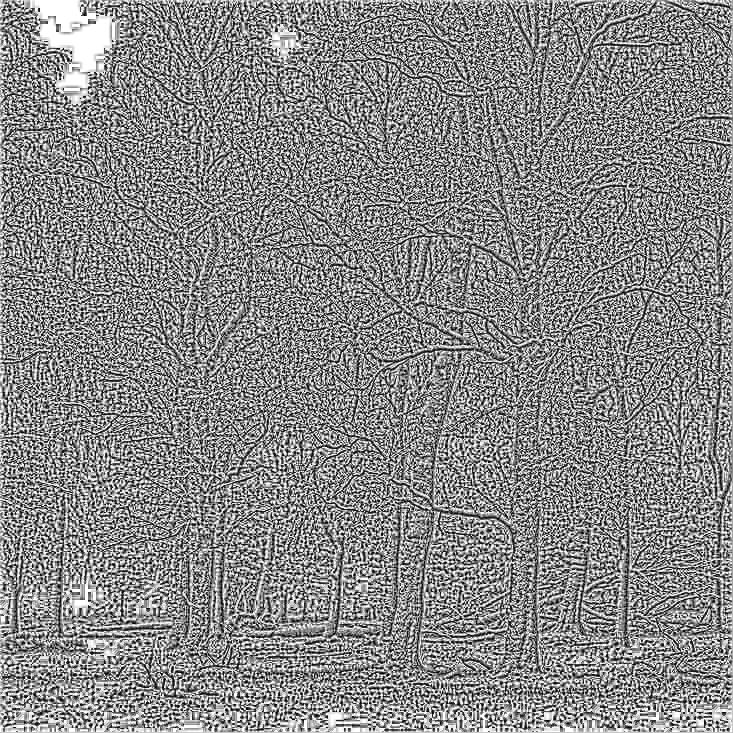
\includegraphics[width=\textwidth]{LC2_local_7.jpg}
        \caption{7x7 local histogram}
    \end{minipage}
    % \hfill
    \begin{minipage}[b]{0.45\textwidth}
        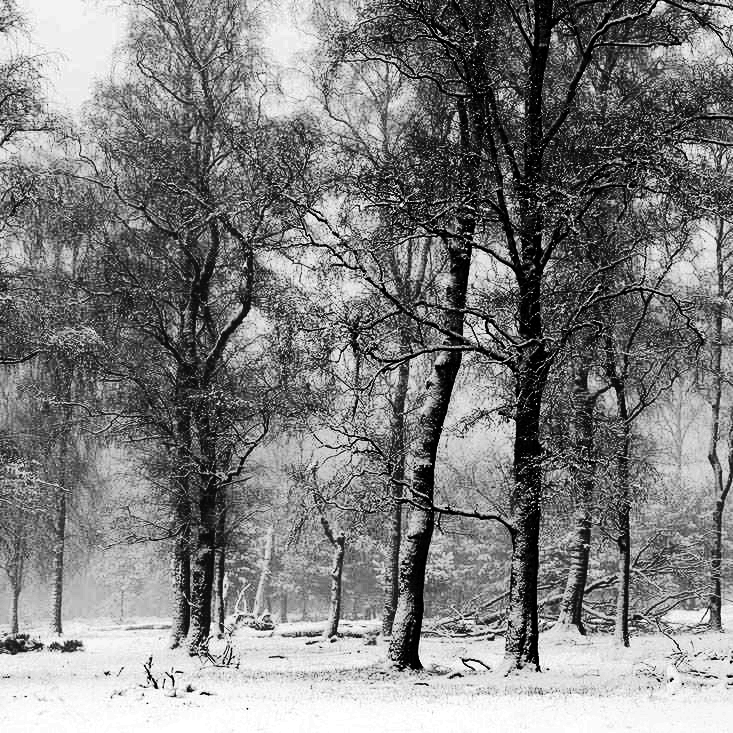
\includegraphics[width=\textwidth]{LC2_global.png}
        \caption{Global histogram}
    \end{minipage}
    % \hfill
\end{figure}

Here, the 7X7 bin shows only the outline of the tree edges, and does not have any region of advantage in comparison to the global histogram. 

A very far stretch would be considering the fine edges of the local histogram.

\newpage
\begin{figure}[!htb]
    \centering
    \begin{minipage}[b]{0.45\textwidth}
        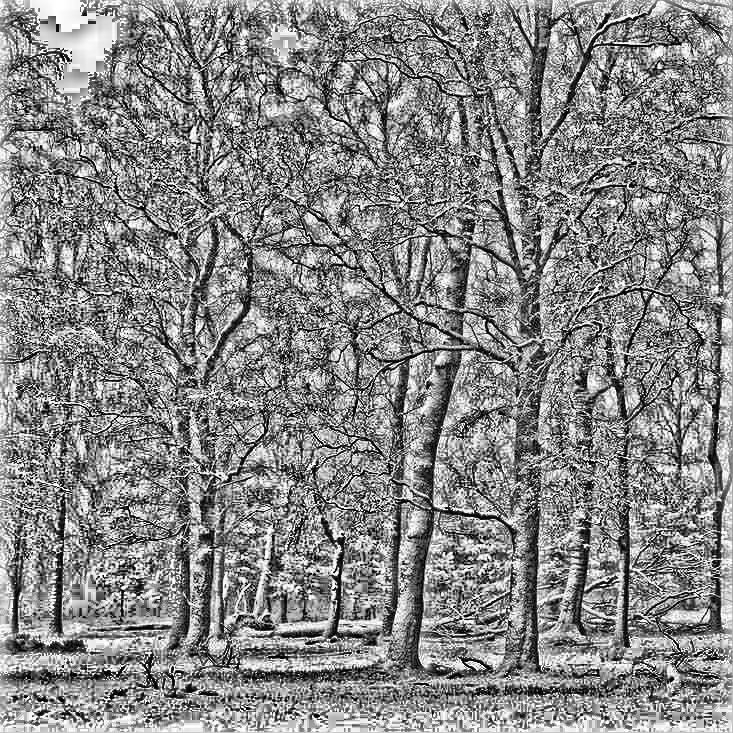
\includegraphics[width=\textwidth]{LC2_local_31.jpg}
        \caption{31x31 local histogram}
    \end{minipage}
    % \hfill
    \begin{minipage}[b]{0.45\textwidth}
        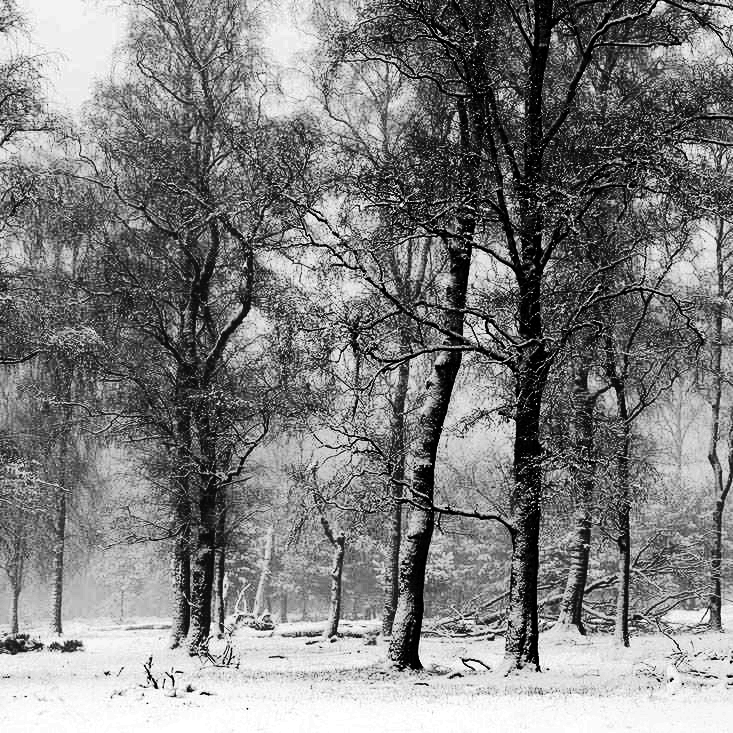
\includegraphics[width=\textwidth]{LC2_global.png}
        \caption{Global histogram}
    \end{minipage}
    % \hfill
\end{figure}

Now, the 31X31 local histogram is better than the previous 7X7 bin local histogram, and in the lower regions of the tree the edges got darker, whereas it is faded in the global histogram.

\begin{figure}[!htb]
    \centering
    \begin{minipage}[b]{0.45\textwidth}
        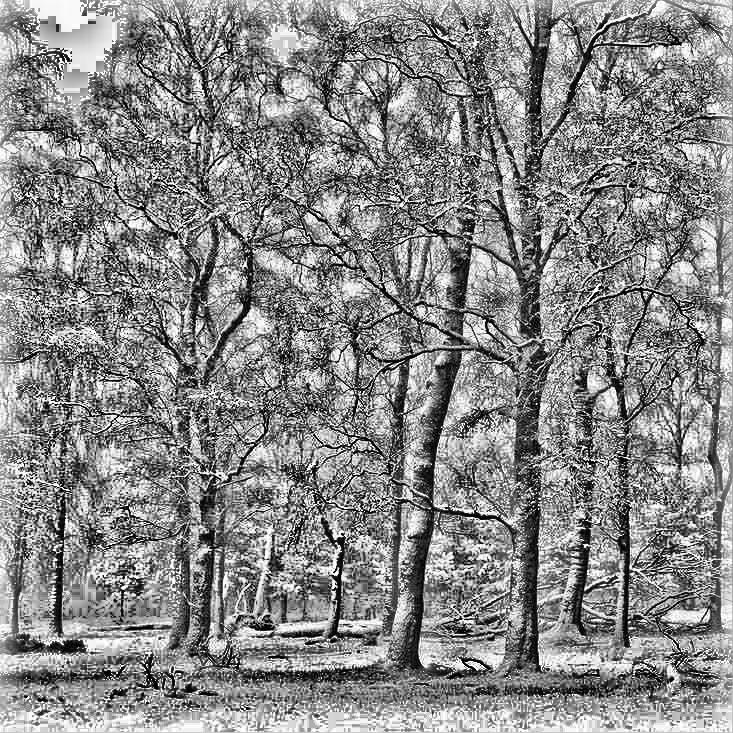
\includegraphics[width=\textwidth]{LC2_local_51.jpg}
        \caption{51x51 local histogram}
    \end{minipage}
    % \hfill
    \begin{minipage}[b]{0.45\textwidth}
        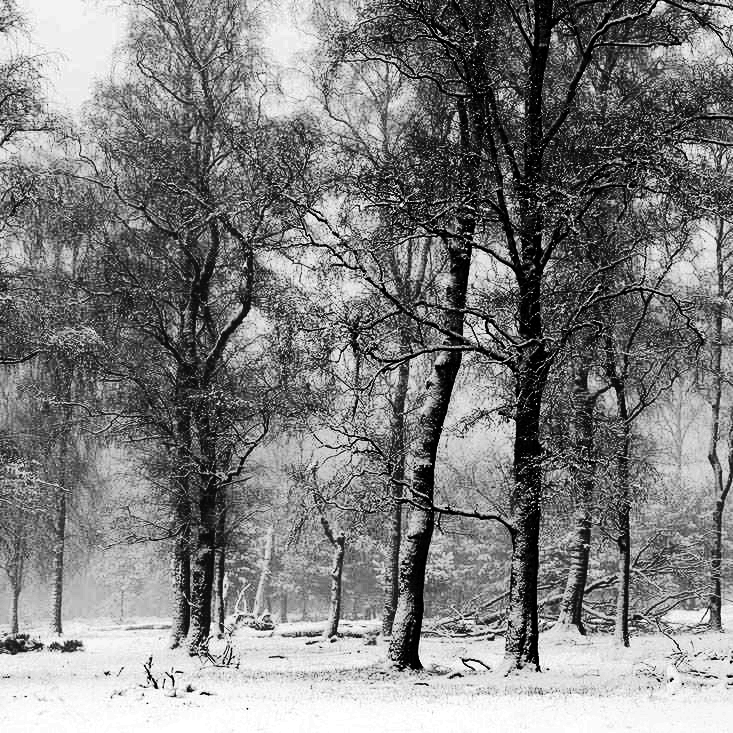
\includegraphics[width=\textwidth]{LC2_global.png}
        \caption{Global histogram}
    \end{minipage}
    % \hfill
\end{figure}

In the 51X51 bin local histogram, the tree outlines and the ground look very crisp and sharp as compared to the global histogram where it appears as low contrast, whereas it is appropriatly fine in local histogram.

\newpage
\begin{figure}[!htb]
    \centering
    \begin{minipage}[b]{0.45\textwidth}
        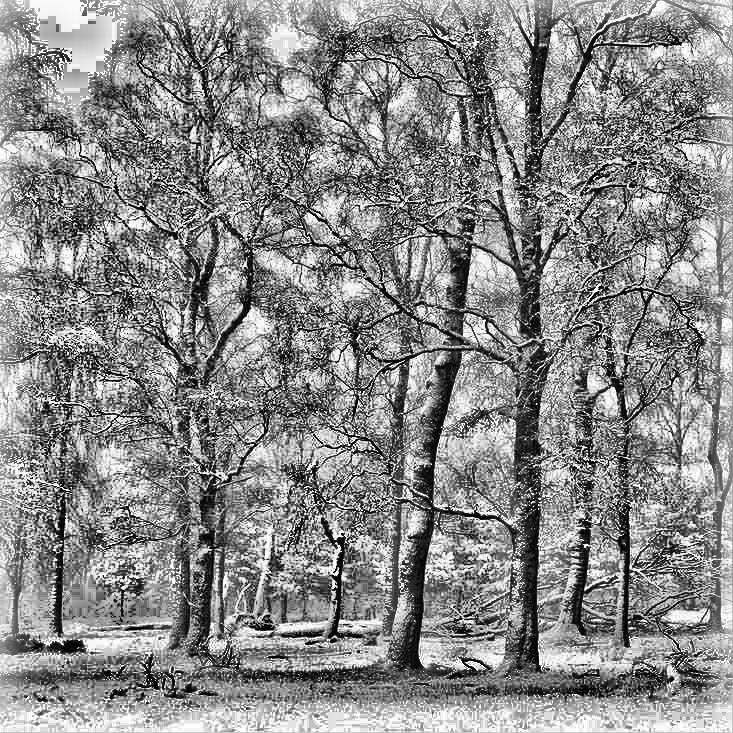
\includegraphics[width=\textwidth]{LC2_local_71.jpg}
        \caption{71x71 local histogram}
    \end{minipage}
    % \hfill
    \begin{minipage}[b]{0.45\textwidth}
        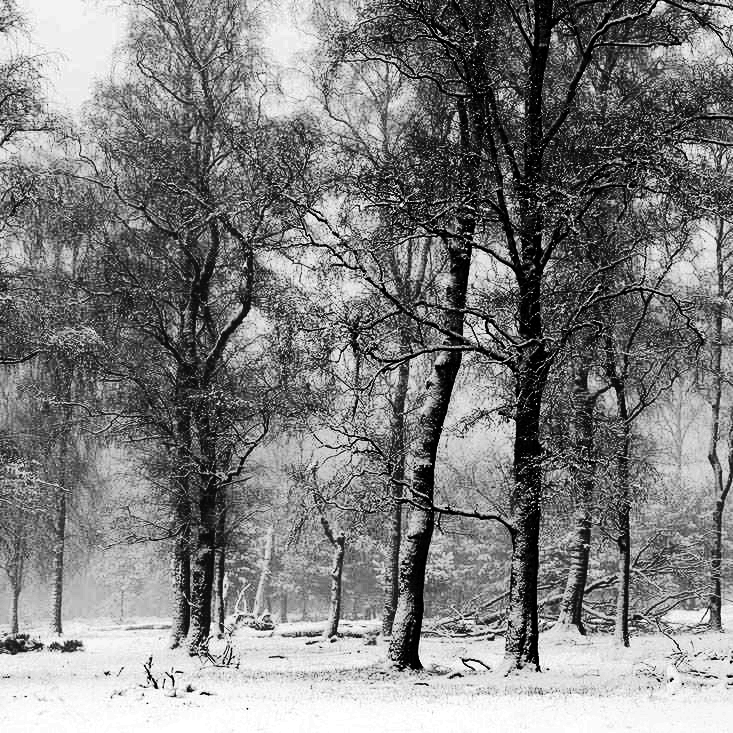
\includegraphics[width=\textwidth]{LC2_global.png}
        \caption{Global histogram}
    \end{minipage}
    % \hfill
\end{figure}

Here, in the 71X71 histogram, the trees in the background are also much clearer than that observed through the global histogram. And, whatever advantages we observed in the previous bins also hold true for this case on comparison with the global histogram.

\subsubsection*{Conclusion}

On observing the image as a whole, the global histogram equalization performs better, but local histogram equalization specialises in the finer aspects of the image that is missed by the global histogram as we have observed in all the above analysis images.


\end{document}